%----------------------------------------------------------
% PACKAGES AND THEMES
%----------------------------------------------------------
\documentclass[aspectratio=169,xcolor=dvipsnames,handout]{beamer}

\usetheme{Darmstadt}
\usecolortheme{seahorse}
\setbeamercovered{transparent}

\usepackage{kotex}
\usepackage{hyperref}
\usepackage{graphicx, array, adjustbox, makecell}
\usepackage{booktabs, multicol, multirow}

%\usepackage{fontspec}
%\setmainfont{Times New Roman}
%\setmainhangulfont{NanumGothic}

\usepackage{newunicodechar}
\newunicodechar{•}{$\cdot$}
\newunicodechar{➔}{$\implies$}
\newunicodechar{∴}{$\therefore$}
\newunicodechar{∵}{$\because$}

%----------------------------------------------------------
% TITLE PAGE
%----------------------------------------------------------
\title{의사결정참가의 주요 제도}
\subtitle{노사관계의 이론과 실제}
\author{오성재}
\institute[CNU]
{\relax
    충남대학교 경제학과
    }
\date{2024년 10월 14일}

%----------------------------------------------------------
\begin{document}
%----------------------------------------------------------

\frame{\titlepage}

\begin{frame}{목차}
    \small
    \tableofcontents[hideallsubsections]
\end{frame}

\section{품질관리분임조}

\begin{frame}
    \frametitle{개관}
    \begin{block}{품질관리분임조 (quality control: QC)}
        소규모의 종업원집단이 정기적으로 모임을 갖고 품질향상 등 작업장에서의 문제해결을 도모하는 제도
    \end{block}
    \begin{itemize}[<+->]
        \item 기존의 조직의 권한과 제도 그리고 위계질서와 상충되지 않고, 기존의 조직에 덧붙여서 그 활동이 이루어지는 경영참가제도 (off-line)의 한 종류.
        \item 5--15명으로 구성
        \item 상부 관리자들의 통제나 간섭 없이, 자체 내에서 분임조장을 중심으로 운영.
        \item QC 조원들이 자치적으로 당면 문제점 제기. 해결방안과 실천방법 논의 및 실행.
        \item 1910년대 미국에서 시작되었으나 1950년대 일본기업이 본격적으로 실시
        \item 1970년대 다시 주목 받기 시작하였으며 우리나라는 1980년대 도입
    \end{itemize}
\end{frame}

\begin{frame}[allowframebreaks]
    \frametitle{시행방법}
    \begin{enumerate}[<+->]
        \item 도입결정
        \begin{itemize}[<+->]
            \item 상의하달식으로 처음 도입
            \item 도입결정 후 자발적 참여자 모집, 자체적으로 안건 및 진행방식 결정
            \item 중간관리자가 소외되는 현상 발생
        \end{itemize}
        \item 교육훈련
        \begin{itemize}[<+->]
            \item 교육훈련이 중요, 특히 전문가에게 3--4일간의 교육훈련 실시
            \item 교육훈련 내용: 단체토의 요령, 합의도출방법, 문제해결능력 배양 등
        \end{itemize}
        \item 진행방식 및 권한
        \begin{itemize}[<+->]
            \item 모임은 주 1회, 1회 1--2시간 정도
            \item 구성원은 문제해결에 대한 제안사항 작성 및 보고 권한 부여
            \item 단, 제안사항의 시행권한은 상급 관리층에게 주어짐. (제안이 꼭 채택되지는 않음)
        \end{itemize}
    \framebreak\relax
        \item 실시과정
        \begin{enumerate}[<+->]
            \item QC의 필요성 인식 및 지지 확보
            \item QC 목표 설정
            \item 중간관리자 교육훈련
            \item 종업원대상 QC 홍보 및 모집된 QC 구성원 교육훈련
            \item QC구성, 목표 확립
            \item 리더선출 및 역할분담
            \item QC의 공식적 선포
            \item 경과 후 QC 평가 및 개선
        \end{enumerate}
    \end{enumerate}
\end{frame}

\begin{frame}
    \frametitle{효과}
    \begin{itemize}[<+->]
        \item 노동자들은 QC를 통해 조직 내의 문제점을 발견하고, 조직의 전반적인 생산과정 및 작업수행과정에 대한 안목이 넓어짐 $\implies$ 장기적으로 생산성 향상 도모
        \item 하의상달의 의사소통구조를 원활히 하여 기업의 의사소통구조를 점진적으로 개선.
        \item 말단 사원들이 경영자의 방침과 고정을 이해하고 회사의 당면 문제점을 파악함.
        \begin{itemize}[<+->]
            \item 상의하달의 의사소통이 자연스럽게 이루어짐.
        \end{itemize}
        \item QC의 시행으로 문제해결, 대인관계 개선, 통계처리방법 등에 대한 훈련을 받아 장기적으로 생산성 향상에 기여.
        \item $\therefore$ QC는 효과가 미흡하지만 긍정적이며 구성원의 주관적 평가에서 바람직한 결과를 보여줌. 단, 경영성과의 획기적 개선을 가져오지는 않음.
    \end{itemize}
\end{frame}

\section{노사합동위원회}%

\begin{frame}[allowframebreaks]
    \frametitle{참여동기}
    \begin{block}{노사합동위원회 (union-management joint committee)}
        유노조 기업에서 노조의 경영참가를 통해 기업의 경쟁력을 높이고 노조원의 고용안정을 도모하기 위한 제도
    \end{block}
    \begin{itemize}[<+->]
        \item 노동조합이 주체가 되어 생산성 향상, 품질향상, 근무환경개선 등을 목표로 기존 제도의 문제점을 개선하는 방안을 찾는 경영참가제도 (유노조 기업에서 이루어진다는 특징)
        \item 실시과정: 기업차원의 노사합동위원회 구성 ➔ 공장 및 작업장별 노사합동위원회 구성 ➔ 참여에 대한 관심 증대 ➔ 다른 유형의 경영참가제도 도입 (성과배분제, 현장자율경영팀 등)
    \framebreak\relax
        \item 노동조합측의 참여동기:
        \begin{itemize}[<+->]
            \item 기업의 경쟁력 저하 및 위기 시 노사협조를 통한 고용안정도모 가능.
            \item 단체협상이 갖지 못하는 장점이 있기 때문에.
        \end{itemize}
        \item 사용자측의 참여동기:
        \begin{itemize}[<+->]
            \item 회사 경쟁력 강화 수단.
            \item 노조와의 대립적 관계 개선.
            \item 상대방에 대한 이해의 폭이 넓어짐.
            \item 상설기구로 필요 시 언제든지 협조적 분위기에서 토의 가능.
        \end{itemize}
    \end{itemize}
\end{frame}


\begin{frame}[allowframebreaks]
    \frametitle{사전 준비사항}
    \begin{enumerate}[<+->]
        \item 교육훈련
        \begin{itemize}[<+->]
            \item 실시 전에 노사 양측의 참가자들에게 교육훈련 실시
            \item 노사협조의 이론 소개, 노사합동의 문제해결기법, 정보공유, 회사의 경영상태 등
            \item 외부 컨설턴트의 도움으로 실시하며 1일--1주일 소요
        \end{itemize}
        \item 노사간 합의
        \begin{itemize}[<+->]
            \item 합의사항을 단체협약 또는 양해각서로 작성
            \item 단체협약에서 충분히 논의된 사항 배제
            \item 위원회 활동의 결과로 노조원들이 해고되지 않도록 함. 
            \item $\because$ 조합원의 지지를 받을 수 없으며 노사협조 정신에 위배
        \end{itemize}
    \framebreak\relax
        \item 외부 컨설턴트 활용
        \begin{itemize}[<+->]
            \item 노사합동위원회에 대한 경험과 지식을 가진 전문가로 위원회의 도입에서부터 진행 및 중재 등의 역할 수행 $\implies$시행착오 제거, 시행상의 문제점 즉각적인 해결
            \item 연구결과에서도 컨설턴트의 고용은 성공적인 정착에 긍정적 효과
            \item 단, 위원회 운영기간 내내 컨설턴트의 의존은 노사양측의 자율적 유지능력을 위축
        \end{itemize}
    \end{enumerate}
\end{frame}

\begin{frame}[allowframebreaks]
    \frametitle{구조 및 활동}
    \begin{itemize}[<+->]
        \item 기존 조직구성과 권한에 상충되지 않고 기존의 조직에 덧붙여서 그 활동이 이루어지는 off-line형태
        \item 기존 조직구조에 대응하는 여러 계층의 위원회 구성. $\because$ 기업과 노조의 위계질서 고려
        \begin{itemize}[<+->]
            \item 기업차원의 노사합동위원회
            \item 공장별 노사합동위원회
            \item 작업장별 노사합동위원회
        \end{itemize}
    \framebreak\relax
        \item  단계별 노사합동위원회의 구성과 논의사항
        \begin{itemize}[<+->]
            \item 작업장별 노사합동위원회: 중간관리자와 노조의 대의원 또는 종업원대표로 구성
            \begin{itemize}[<+->]
                \item 작업장 업무와 관련된 문제점 해결, 산업안전 사항, 생산비 절감, QC와 비슷한 활동
            \end{itemize}
        \item 공장별 노사합동위원회: 공장의 경영층과 노조지부의 간부, 종업원 대표로 구성
            \begin{itemize}[<+->]
                \item 생산성 향상, 품질개선, 작업환경개선, 종업원교육훈련, 납품업자 관리 등 논의
            \end{itemize}
        \item 기업차원의 노사합동위원회: 최고 경영자와 노조본부의 간부로 구성
            \begin{itemize}[<+->]
                \item 투자계획·제품전략·공장신설 등 논의
                \item 전략적 의사결정에 참여 (participation in strategic decision-making)이라고도 함
            \end{itemize}
        \end{itemize}
    \end{itemize}
\end{frame}

\begin{frame}
    \frametitle{권한}
    \begin{itemize}[<+->]
        \item 노사합동위원회: 의사결정구조를 근본적으로 변경하지 않으며 (off-line) 자문기구로서의 역할 수행
        \begin{itemize}[<+->]
            \item $\therefore$ 공식적 의사결정기구로서의 성격 미흡
        \end{itemize}
        \item 노사합동위원회의 결정: 양측 대표간의 합의에 의해 이루어져야
        \begin{itemize}[<+->]
            \item $\because$ 다수결방식은 노사협조의 정신을 해치고 노사 쌍방간에 대결구조 조장 우려
        \end{itemize}
        \item 합의된 사항을 해당 부서에 통보 및 실시: 합의사항에 대한 경영층 또는 조합원의 반발 가능성
        \begin{itemize}[<+->]
            \item $\implies$ 합의사항을 이행하지 못하는 상황 발생 가능
            \item 노사쌍방이 중요 의사결정권을 실제로 행사하는 인물이 위원회에 참여하도록 하여야
        \end{itemize}
    \end{itemize}
\end{frame}

\begin{frame}
    \frametitle{효과제고 고려사항}
    \begin{itemize}[<+->]
        \item 노사합동위원회가 성공하기 위해서는 필요한 환경요건
        \item 노사 양측에서 실제 의사결정권을 가진 인물들이 노사합동위원회의 위원으로 참여
        \item 노사합동위원회의 목표에 대해 노사간의 합의에 의해서 사전에 명확히 정해지는 것이 바람직 함
        \item 경험 많고 능력 있는 외부 컨설턴트의 확보
        \item 여러 단계의 노사합동위원회의 역할이 서로 상충되지 않도록 조정하는 작업 필요
        \item 경영스타일과 기업문화가 노조의 경영참가를 수용할 수 있는 참여적 조직이 바람직 함
        \item 전국규모의 노조본부의 정책과 노조원들의 태도가 노조의 경영참가에 긍정적이거나 최소한 반대하지 않는 자세를 보일 경우
    \end{itemize}
\end{frame}

\begin{frame}
    \frametitle{효과}
    \begin{itemize}[<+->]
        \item 기대효과
        \begin{itemize}[<+->]
            \item 노사 쌍방이 서로의 입장에 대한 이해가 깊어짐, 장기적으로 협조적 고용관계 정착
            \item 합의•도출된 의사결정은 종업원의 입장이 반영된 것이므로 지지 받을 가능성 높음
            \item 피고용인의 요구사항이 반영되어 작업환경에 긍정적 영향 ➔ 직무만족도 향상
            \item 전반적 생산과정의 효율화가 이루어져 장기적인 생산성 및 품질향상 기대
        \end{itemize}
        \item 실증연구 결과
        \begin{itemize}[<+->]
            \item 협력적 고용관계 증진, 제품 및 서비스 품질 향상, 생산성 및 경쟁력 제고 등 기업과 피고용인에게 대체로 긍정적인 영향을 줌
            \item 특히, 경영성과 향상보다는 고용관계의 증진에 더 큰 영향 (∵ 노사합동위원회 성격상 자문기구의 성격이 강하기 때문에)
            \item 노동조합이 전략적 의사결정에 실질적으로 참여할 경우 경영성과와 고용관계의 증진에 긍정적 기여
        \end{itemize}
    \end{itemize}
\end{frame}

\section{현장자율경영팀}%

\begin{frame}[allowframebreaks]
    \frametitle{개관}
    \begin{block}{현장자율경영팀 (self-managing work team, self-directed team, autonomous work team)}
        15명 미만의 종업원들이 팀을 구성하여 감독자 없이 생산에 관한 결정을 스스로 내리며 독자적으로 생산활동을 수행하는 경영참가제도의 한 형태
    \end{block}
    \begin{itemize}[<+->]
        \item 현장자율경영팀의 구성 목적:
            \begin{itemize}[<+->]
                \item 집단 구성원의 사회적 욕구를 충족시켜 협동시스템을 구축하고,
                \item 개개 종업원의 노하우가 공동작업을 통해 구성원에게 공유될 수 있도록 하며
                \item 개인의 성장욕구를 충족시켜 직무만족이나 기업의 성과를 높이는 것.
            \end{itemize}
        \item 도입한 대표적 다국적 기업: Saturn, Xerox, FedEx, TRW, P\&G.
        \item 국내기업으로는 LG전자, LG필립스 등이 있으며 긍정적 효과를 거두고 있음
    \end{itemize}
\end{frame}

\begin{frame}[allowframebreaks]
    \frametitle{시행방법}
    \begin{itemize}[<+->]
        \item 도입과정
        \begin{itemize}[<+->]
            \item 최고경영층의 결정으로 도입:
            \begin{itemize}[<+->]
                \item ∵ 중간관리자의 권한이 상당부분 하부로 이양되므로 도입의 저항세력으로 작용
                \item ∵ 하부구성원 중에도 도입에 부담을 느낄 수 있으므로
            \end{itemize}
        \item 기존의 경영방식과 기업문화를 고려하여 세밀한 준비가 바람직
        \end{itemize}
    \item 구성
        \begin{itemize}[<+->]
            \item 작업성격이 강한 부서를 중심으로 우선 적용 ➔ 결과에 따라 타 부서로 확대 적용
            \item 적정한 팀원 수 유지가 바람직. ∵ 팀 구성원이 너무 많은 경우, 팀워크 형성 곤란 및 구성원간 응집력 저하 등
        \end{itemize}
    \framebreak\relax
    \item 교육훈련
        \begin{itemize}[<+->]
            \item 철저한 교육훈련 필요
            \item 기술습득훈련: OJT를 통한 기술습득
            \item 대인관계 개선훈련: 상호간의 원만한 인간관계 형성 및 합의에 의한 집단의사결정 능력 배양
        \end{itemize}
    \item 도입 시 유의사항
        \begin{itemize}[<+->]
            \item 각 직무간 상호보완적인 연관성이 있는 작업조직에서 실시
            \item 성장욕구가 강하고 자율적인 직무수행을 선호하는 종업원집단에서 실시
            \item 철저한 교육훈련 실시
        \end{itemize}
    \end{itemize}
\end{frame}

\begin{frame}
    \frametitle{효과}
    \begin{itemize}[<+->]
        \item 자율적 작업집단은 성과 및 생산성 향상에 긍정적 영향
        \item 현장자율경영팀 구성원들이 다른 구성원보다 높은 직무만족도를 보임
        \item 종업원들의 결근율이 줄어듦
        \item 실증연구 결과 현장자율경영팀이 조직과 그 구성원에게 긍정적인 영향을 줌
    \end{itemize}
\end{frame}

\section{근로자이사제도}

\begin{frame}
    \frametitle{개관}
    \begin{block}{근로자이사제도 (employee representation on board)}
        노동조합의 대표 혹은 종업원 대표가 기업의 이사회 (board of directors)에 참석하여 공식적으로 기업의 최고의사결정과정에 참여하는 제도
    \end{block}
    \begin{itemize}[<+->]
        \item 유럽 국가: 산업민주주의 실현을 위한 한 수단으로서 법률에 의하여 강제되는 경우가 많음
        \item 미국: 당사자 자율주의 (voluntarism)를 지향하고 있어 노사간의 합의에 의해서 실시되는 것이 대부분
    \end{itemize}
\end{frame}

\begin{frame}[allowframebreaks]
    \frametitle{유형}
    \begin{itemize}[<+->]
        \item 유럽의 근로자이사제
        \begin{itemize}[<+->]
            \item 1951년 독일에서 시작 스웨덴•오스트리아•노르웨이•베네룩스3국 등으로 전파
            \item 유럽통합 이후 실시 계획 (∵ 산업민주주의의 실현을 위해)
            \item 실시대상, 과정 등에 대한 세밀하게 법률로 규정되어 있음
            \item 일정규모 이상의 기업은 의무적으로 실시하도록 규정
            \item 이원적 이사회 (독일, 네덜란드 등)의 경우 근로자이사는 한 이사회에만 포함
            \item 일원적 이사회 (아일랜드, 스웨덴 등)의 경우 단일 이사회 구성원으로 활동
        \end{itemize}
    \framebreak\relax
        \item 미국의 근로자이사제
        \begin{itemize}[<+->]
            \item 당사자 자율주의 존중 ➔ 법률로 강제되지 않으며 노사간 합의에 의해 시행
            \item 1980년대 초부터 노사협상에서 노조의 양보를 얻는 대신 노조에 이사회 의석 할당 (예: Chrysler, East Airlines, Pan American Airlines 등)
            \item 경영위기 시 노조의 협조를 통해 성과개선을 도모
            \item 근로자이사 수가 적어 의사결정에 대한 영향력이 유럽에 비해 상대적으로 제한적
        \end{itemize}
    \end{itemize}
\end{frame}

\begin{frame}[allowframebreaks]
    \frametitle{효과}
    \begin{itemize}[<+->]
        \item 근로자이사제의 긍정적 성과:
        \begin{itemize}[<+->]
            \item 노사간에 정보공유
            \item 의사결정과정에서 노동문제의 중요성 부각. 특히, 인사관리 및 고용관계에 대한 의사결정 시 근로자이사의 의견이 많이 반영됨
            \item ➔ 근로자이사제의 실시로 기업의 의사결정방식이 피고용인의 입장을 존중하는 방향으로 바뀌고 전반적인 영향 강화되었음
        \end{itemize}
    \framebreak\relax
        \item 근로자이사제의 부정적 성과:
        \begin{itemize}[<+->]
            \item 산업민주주의의 상징적 역할이 있을 뿐 기업 의사결정구조에 별다른 영향을 주지 못함
            \item $\because$ 상대적으로 소수인 근로자이사 수 ➔ 의사결정에 중요한 영향을 주지 못함
            \item 근로자이사가 이사회의 본질적 기능 (주주의 권리 대변)을 수행하며 역할갈등 발생
            \item 경영인보다 상대적으로 경영 전문지식 결여
        \end{itemize}
    \item 생산성, 품질효율성, 종업원 태도 등에 미약한 영향: 산업민주주의 또는 노사협조 등의 상징적 역할
    \item 일관된 결과가 나타나지 않음. (∵ 국가별 고용관계시스템의 차이에서 기인된 것으로 판단됨)
    \end{itemize}
\end{frame}

\section{노사협의회}

\begin{frame}[allowframebreaks]
    \frametitle{개관}
    \begin{block}{노사협의회}
        근로자와 사용자가 참여와 협력을 통하여 근로자의 복지증진과 기업의 건전한 발전을 도모함을 목적으로 구성하는 협의기구 (『근로자참여 및 협력증진에 관한 법률』제3조 제1항)
    \end{block}
    \begin{itemize}[<+->]
        \item 작업장 단위에서 사용자와 근로자가 작업에서의 문제해결과 공동관심사를 협의하는 제도
        \begin{itemize}[<+->]
            \item 노사대표로 구성: 한국, 프랑스, 벨기에 등 ∴ 노사협의회 (labor-management committee)
            \item 근로자 대표만으로 구성: 독일, 오스트리아, 네덜란드, 스페인 등 ∴ 작업장평의회 (works council)
            \item 실시 강제여부: 일부 유럽과 아시아 등 법률로 강제, 영국과 미국은 노사간의 합의로 실시
        \end{itemize}
    \framebreak\relax
        \item 노사협의회를 운영함에 있어서 피고용인과 사용자는 상호신의를 기초로 성실하게 협의하고, 피고용인의 복지증진과 기업의 건전한 발전을 도모해야 함
        \item 특징
        \begin{itemize}[<+->]
            \item 법령에 의해 사업 또는 사업장단위로 그 설치와 운영이 강제
            \item 노사협의의 기능은 경영관리적 내지 경영참가적 성격
            \item 피고용인의 과반수로 조직된 노동조합이 있는 경우 노동조합의 대표자와 그 노동조합이 위촉하는 자로 하여금 근로자대표위원을 구성하도록 함
        \end{itemize}
    \end{itemize}
\end{frame}

\begin{frame}[allowframebreaks]
    \frametitle{단체교섭과의 관계}
    \begin{itemize}[<+->]
        \item 노사협의회: 평화적 처리가 전제
        \begin{itemize}[<+->]
            \item 경영참가라는 생산수단의 운영에 의한 가치생산과정에 있어서 노사 이해공통적 관계의 해결을 본질적 과제로 봄 ➔ 파이 (pie)의 생산에 참여
        \end{itemize}
        \item 단체교섭: 쟁의권을 전제
        \begin{itemize}[<+->]
            \item 가치배분과정에서 노사간 이해대립적 관계의 해결을 본질적 과제로 봄 ➔ 파이 배분 참여
        \end{itemize}
    \end{itemize}
    \framebreak\relax
    \begin{table}
        \centering
        \resizebox{.8\textwidth}{!}{\relax
            \begin{tabular}{p{2cm} p{7cm} p{7cm}}
\toprule
 & \textbf{노사협의회} & \textbf{단체교섭} \\
\midrule
\textbf{목적} & 노사공동의 이익증진과 산업평화 도모 & 근로조건의 유지와 개선 \\ \midrule
\textbf{배경} & 노동조합의 설립 여부와 관계없이 쟁의행위라는 위협의 배경없이 진행 & 노동조합 및 기타 노동단체의 존립을 전제로 하고 자력구제로서의 쟁의의 배경 \\ \midrule
\textbf{당사자} & 근로자 대표와 사용자 & 노동조합의 대표자와 사용자 \\ \midrule
\textbf{대상사항} & 기업의 경영이나 생산성 향상 등과 같이 노사간 이해가 공통 & 임금 근로시간 기타 근로조건에 관한 사항처럼 이해가 대립 \\ \midrule
\textbf{결과} & 법적 구속력 있는 계약체결이 이루어지지 않을 수 있음 & 단체교섭이 원만히 이루어진 경우 단체협약 체결 \\
\bottomrule
\end{tabular}

        }
        \caption{노사협의회와 단체교섭}
    \end{table}
    \framebreak\relax
    \begin{itemize}[<+->]
        \item 노사협의회와 단체교섭과의 관계:
        \begin{itemize}[<+->]
            \item 분리형: 단체교섭과 노사협의회를 별도의 제도로 분리하여 운영하는 방식
            \item 연결형: 단체교섭과 노사협의회를 각각 별도의 제도로 분리하여 운영하지만 양 제도가 유기적인 관련성을 맺고 운영하는 방식
            \item 대체형: 단체교섭과 노사협의회 양 제도를 서로 구분하지 않고 노사협의회에서 단체교섭 사항까지 논의하는 운영방식. 
                \begin{itemize}[<+->]
                    \item 상호이익이 되는 관심사를 다루는 노사협의회가 대립적인 사안이 많은 상호단체교섭사항을 다루게 되어 갈등구조로 흐르기 쉽다는 단점.
                \end{itemize}
        \end{itemize}
    \end{itemize}
\end{frame}

\begin{frame}
    \frametitle{구성}
    \begin{itemize}[<+->]
        \item 『근로자참여 및 협력증진에 관한 법률』: 30인 이상의 사업장에서 반드시 구성해야
        \item 노사협의회 구성
        \begin{itemize}[<+->]
            \item 근로자와 사용자를 대표하는 동수의 위원으로 구성하되 그 수는 각 3--10명 이내
            \item 의장은 위원 중에서 호선
            \item 근로자위원: 근로자 직선이 원칙. 3년 연임 가능. 
                \begin{itemize}[<+->]
                    \item 단, 근로자의 과반수로 조직된 노동조합이 있는 경우에는 노조 대표자와 그 노동조합이 위촉. 
                    \item 노동조합원이 과반수를 넘지 못하거나 노동조합이 없는 경우에는 근로자의 직접·비밀·무기명투표로 선출
                \end{itemize}
            \item 비상임·무보수
        \end{itemize}
    \item 사용자는 근로자위원에게 직무수행과 관련하여 불이익한 처분을 하면 안됨 
    \end{itemize}
\end{frame}

\begin{frame}[allowframebreaks]
    \frametitle{운영 및 임무}
    \begin{enumerate}[<+->]
        \item 운영
        \begin{itemize}[<+->]
            \item 3개월마다 정기적으로 개최, 필요 시 임시회의 개최
            \item 과반수 이상의 출석으로 개최하고 출석위원 3분의 2 이상의 찬성으로 의결
        \end{itemize}
        \item 임무: 보고사항, 협의사항, 의결사항
    \end{enumerate}
    \begin{itemize}[<+->]
        \item 보고사항: 사용자가 협의회에서 보고 설명하여야 사항
        \begin{itemize}[<+->]
            \item 주로 경영정보공유의 성질로서 경영계획 전반 및 실적 사항, 분기별 생산계획과 실적 사항, 인력계획, 기업의 경제적 재정적 상황 등
        \end{itemize}
    \framebreak\relax
    \item 협의사항: 협의하여 합의에 도달할 수 있는 사항
        \begin{itemize}[<+->]
            \item 생산성 향상과 성과배분, 근로자의 채용 배치 및 교육훈련, 노동쟁의의 예방, 근로자의 고충처리, 안전보건 기타 작업환경 개선과 근로자의 건강증진, 인사노무관리의 제도개선.
        \end{itemize}
    \item 의결사항: 사용자가 반드시 협의회의 의결을 거쳐야 한 시행할 수 있는 사항.
        \begin{itemize}[<+->]
            \item 고충처리위원회에서 의결되지 아니한 사항, 각종 노사공동위원회의 설치 등.
            \item 의결이 된 사항은 신속히 공지하고 노사 양측은 성실하게 이행하여야 할 의무 부과.
        \end{itemize}
    \end{itemize}
\end{frame}


\begin{frame}
    \frametitle{고충처리제도}
    \begin{itemize}[<+->]
        \item 고충처리위원: 상시 30인 이상의 근로자를 사용하는 모든 사업 또는 사업장에는 고충처리위원을 둠 (『근로자참여 및 협력증진에 관한 법률』제25조)
        \item 구성: 노사를 대표하여 3인 이내의 위원으로 구성하되 협의회가 설치되어 있는 경우 협의회에서 선임하고 그렇지 않을 경우 사용자가 위촉
        \item 고충 처리: 고충처리위원은 근로자로부터 고충사항을 청취한 때에는 10일 이내에 조치사항 기타 처리결과를 당해 근로자에게 통보하여야 하며 처리가 곤란할 때에는 협의회에 부의하여 협의처리함
        \item 유노조$\cdot$무노조 모두 설치하도록 강제: 피고용인의 권익을 보다 철저히 보호하기 위한 취지
    \end{itemize}
\end{frame}

\section{고성과 작업시스템}

\begin{frame}[allowframebreaks]
    \frametitle{정의}
    \begin{block}{고성과 작업시스템 (High Performance Work Systems; HPWS)}
        노사간의 협력 및 신뢰를 바탕으로 근로자들에게 지식축적, 동기유발 및 열린경영 (또는 경영참가)의 원칙에 입각한 인사노무관리를 통하여 근로자의 자유재량 노력을 극대화함으로써 조직성과의 향상을 도모하는 작업시스템
    \end{block}
    \begin{itemize}[<+->]
        \item 고성과 작업시스템의 3가지 요소
        \begin{enumerate}[<+->]
            \item 지식축적 (Skill-building, Knowledge-building)
            \item 동기유발 (Motivation)
            \item 경영참가 (Communication and Employee involvement)
        \end{enumerate}
    \end{itemize}
    \centering
    \begin{figure}
        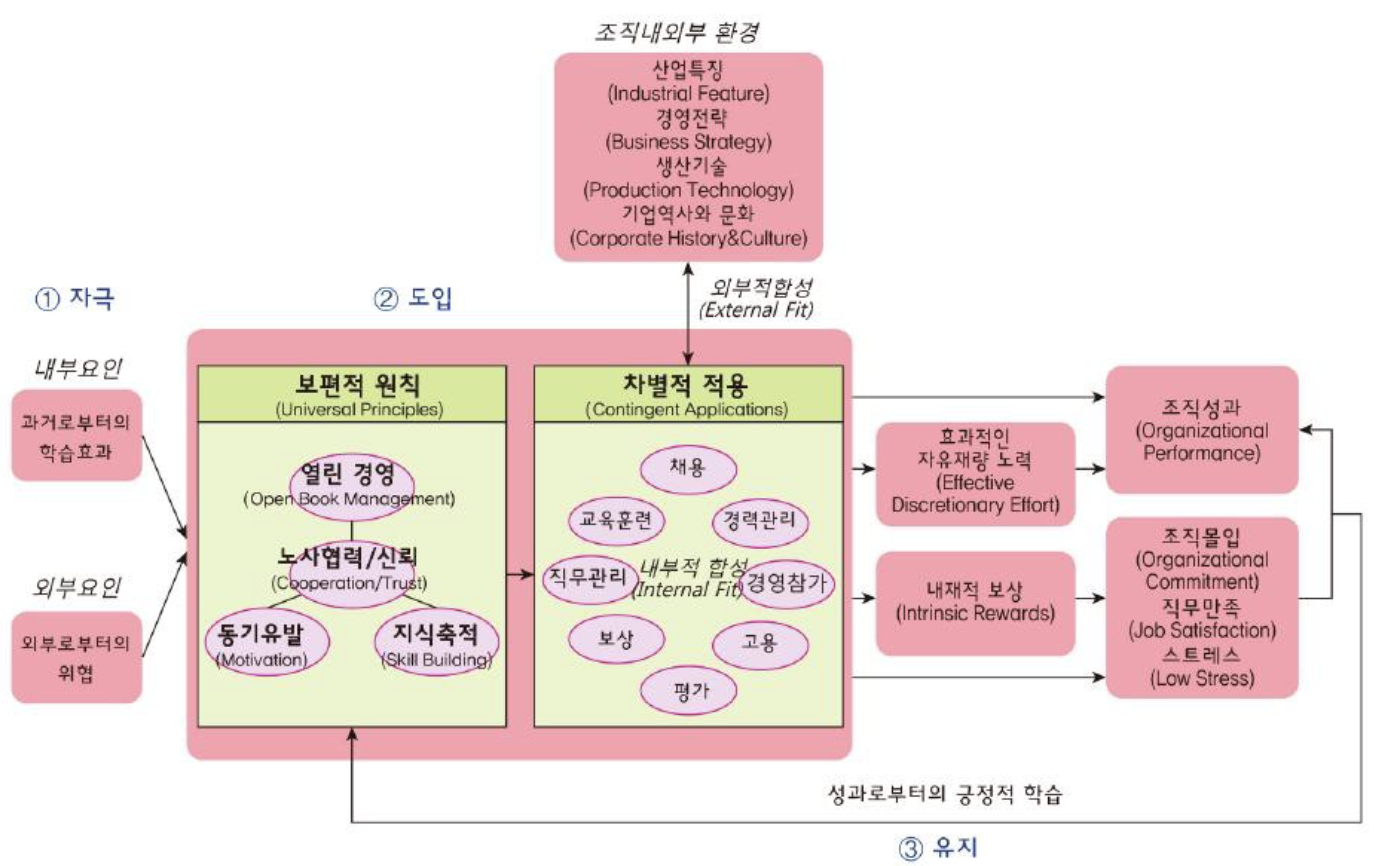
\includegraphics[width=.65\textwidth]{pic/HPWS.png}
        \caption{고성과 작업시스템 통합모형}
    \end{figure}
\end{frame}

\begin{frame}
    \frametitle{적합성 개념}
    \begin{itemize}[<+->]
        \item 내적적합성 (Internal fit): 통일성 있는 고용관계전략을 형성하기 위하여 다양한 고용관계 정책과 관행들이 충분히 통합되어 시너지 효과를 나타내는 상태 및 과정을 의미
        \item 외적적합성 (External fit): 고용관계 시스템이 궁극적으로 조직이 처한 내외부 환경과 전략과 일치하여야 기업의 효율성이 극대화된다는 개념
    \end{itemize}
\end{frame}


%------------------------------------------------
\end{document}
%------------------------------------------------
